% easychair.tex,v 3.4 2015/12/10

\documentclass{easychair}
%\documentclass[EPiC]{easychair}
%\documentclass[debug]{easychair}
%\documentclass[verbose]{easychair}
%\documentclass[notimes]{easychair}
%\documentclass[withtimes]{easychair}
%\documentclass[a4paper]{easychair}
%\documentclass[letterpaper]{easychair}

\usepackage{doc}

% use this if you have a long article and want to create an index
% \usepackage{makeidx}

% In order to save space or manage large tables or figures in a
% landcape-like text, you can use the rotating and pdflscape
% packages. Uncomment the desired from the below.
%
% \usepackage{rotating}
% \usepackage{pdflscape}

% Some of our commands for this guide.
%
\newcommand{\easychair}{\textsf{easychair}}
\newcommand{\miktex}{MiK{\TeX}}
\newcommand{\texniccenter}{{\TeX}nicCenter}
\newcommand{\makefile}{\texttt{Makefile}}
\newcommand{\latexeditor}{LEd}

%\makeindex

%% Front Matter
%%
% Regular title as in the article class.
%
\title{Benchmarks for Verification of Autonomous Vehicles }


% Authors are joined by \and. Their affiliations are given by \inst, which indexes
% into the list defined using \institute
%
\author{
Matthew O'Kelly\inst{1}
\and
    Houssam Abbas\inst{1}
\and
  Aditya Pinapala \inst{1}
\and
 Rahul Mangharam \inst{1}
}

% Institutes for affiliations are also joined by \and,
\institute{
  University of Pennsylvania,
  Philadelphia, PA, U.S.A.\\
  \email{mokelly@seas.upenn.edu, }
  \email{habbas@seas.upenn.edu, }
  \email{pinapala@seas.upenn.edu, and}
  \email{rahulm@seas.upenn.edu}
 }

%  \authorrunning{} has to be set for the shorter version of the authors' names;
% otherwise a warning will be rendered in the running heads. When processed by
% EasyChair, this command is mandatory: a document without \authorrunning
% will be rejected by EasyChair

\authorrunning{O'Kelly, Abbas, Pinapala, and Mangharam}

% \titlerunning{} has to be set to either the main title or its shorter
% version for the running heads. When processed by
% EasyChair, this command is mandatory: a document without \titlerunning
% will be rejected by EasyChair
\titlerunning{Verification Benchmarks for Autonomous Vehicles}

\begin{document}

\maketitle

\begin{abstract}
  In order to ease the lives of authors, editors, and trees, we present an
  easy-to-read guide to the easy-to-use {\easychair} {\LaTeX2e} document style
  class for EasyChair-based electronic and on-paper publishing of workshop and conference
  proceedings.
\end{abstract}

% The table of contents below is added for your convenience. Please do not use
% the table of contents if you are preparing your paper for publication in the
% EPiC series

%\setcounter{tocdepth}{2}
%{\small
%\tableofcontents}

%\section{To mention}
%
%Processing in EasyChair - number of pages.
%
%Examples of how EasyChair processes papers. Caveats (replacement of EC
%class, errors).

%\pagestyle{empty}

%------------------------------------------------------------------------------
\section{Introduction}
\label{sect:introduction}

\begin{itemize}
	\item Need for AV verification
	\item Why it is hard
	\item Contributions/Benchmarks
	\begin{itemize}
		\item Scenario 1: Obstacle avoidance on a sharp curve
		\item Scenario 2: T-Junction
		\item Scenario 3: Obstructed T-Junction
	\end{itemize}
\end{itemize}

%------------------------------------------------------------------------------
\section{State of the Art}
\begin{itemize}
	\item Types of Autonomy
	\item Levels of Abstraction
	\item Verification Methods and Tools
	\begin{itemize}
		\item Control Perspective: Lyapunov Functions
		\item Software Perspective: Model Checking
		\item Logic Perspective: Theorem Proving
	\end{itemize}
\end{itemize}
%------------------------------------------------------------------------------
\section{Models}
\label{sect:model}
\emph{Key new idea:} Examine continuous evolution of ego-vehicle, but only discrete evolution of environment. Give environment grid-based abstraction. We don't know the control inputs for the environment anyway\newline

\noindent \textbf{Vehicle}
\begin{itemize}
	\item Vehicle Dynamics: Bicycle Model
	\item Planning
	\item Perception
	\item Computation and Scheduling
	\item Traffic Participants
\end{itemize}

\noindent \textbf{Traffic Control}
\begin{itemize}
	\item Stop Sign
	\item Speed Limit
	\item Yield
	\item Traffic Light
\end{itemize}

\noindent \textbf{Pedestrians}
\begin{itemize}
	\item Dynamics
	\item Grid based abstraction
	\item Non determinism
\end{itemize}

%------------------------------------------------------------------------------
\section{Scenarios}
\label{sect:scenarios}

The following are the general default parameters {\easychair}
introduces into the typesetting aspect of articles. If you use
\easychair\ for proceedings or other kinds of publishing through
EasyChair, do not alter these -- papers deviating from the formatting
standards will be rejected by EasyChair.
\section{Verification Engines}

\section{Results}

\section{Conclusions}

\begin{enumerate}
\item
The default paper size is US letter. It can be explicitly set to A4 
(\texttt{a4paper}) or letter (\texttt{letterpaper}) paper in the
document class entry, e.g.:\\\verb+\documentclass[a4paper]{easychair}+

\item
The print area for both letter and A4 paper sizes is 145x224 mm. This size
has been selected to allow for inexpensive printing using our current
print-on-demand publisher.

\item
The base font is Computer Modern. The base font size is 10pt. If you
use any other font size, there is no guarantee that the produced
document will look nice or fit into our standard page size.

\item
The references list is condensed. The default bibliography styles, such as
\texttt{plain}, \texttt{abbrv}, and \texttt{alpha}, are suggested.

\item
PNG, JPG, and PDF images are supported, i.e., those that are supported
by the standard \texttt{graphicx} package \cite{graphicx-package}, and
render nicely in online versions of PDF documents.  This document
shows some examples of JPG and PDF images, for example in
Figure~\ref{fig:easychair-logo}. If the papers are designed for
publishing in print, the images should be at least 300dpi in
resolution. 

\end{enumerate}

\subsection{Tables}

Many page overflows happen because of large tables. In many case these
overflows can be easily removed by slightly reducing padding added by
\LaTeX\ to every column. It is controlled by the \LaTeX\ command
\verb|\tabcolsep| whose value by default is 6pt. Even small changes in
the value of this command may give drastic reductions in the width of
tables. This is illustrated in Figure~\ref{fig:tabcolsep} on
page~\pageref{fig:tabcolsep}. Note though that there is no free lunch:
smaller values for this command may result in lower redability.

%------------------------------------------------------------
\begin{figure}[tb]\small
\begin{center}
  \begin{tabular}{lrrrrrrrr}
    \hline
    ATP System            & LTB & Avg  &Prfs & SOTA & \multicolumn{1}{c}{$\mu$} & CYC & MZR & SMO \\
   \hline
    Vampire-LTB 11.0      &  69 & 24.5 &  69 & 0.37 & 28.1 &  23 &  22 &  24 \\
    iProver-SInE 0.7      &  67 & 76.5 &   0 & 0.36 &  8.8 &  28 &  14 &  25 \\
   \hline
  \end{tabular}
\end{center}

\begin{center}\renewcommand{\tabcolsep}{5pt}
  \begin{tabular}{lrrrrrrrr}
    \hline
    ATP System            & LTB & Avg  &Prfs & SOTA & \multicolumn{1}{c}{$\mu$} & CYC & MZR & SMO \\
   \hline
    Vampire-LTB 11.0      &  69 & 24.5 &  69 & 0.37 & 28.1 &  23 &  22 &  24 \\
    iProver-SInE 0.7      &  67 & 76.5 &   0 & 0.36 &  8.8 &  28 &  14 &  25 \\
   \hline
  \end{tabular}
\end{center}

\begin{center}\renewcommand{\tabcolsep}{3pt}
  \begin{tabular}{lrrrrrrrr}
    \hline
    ATP System            & LTB & Avg  &Prfs & SOTA & \multicolumn{1}{c}{$\mu$} & CYC & MZR & SMO \\
   \hline
    Vampire-LTB 11.0      &  69 & 24.5 &  69 & 0.37 & 28.1 &  23 &  22 &  24 \\
    iProver-SInE 0.7      &  67 & 76.5 &   0 & 0.36 &  8.8 &  28 &  14 &  25 \\
   \hline
  \end{tabular}
\end{center}

\begin{center}\renewcommand{\tabcolsep}{1pt}
  \begin{tabular}{lrrrrrrrr}
    \hline
    ATP System            & LTB & Avg  &Prfs & SOTA & \multicolumn{1}{c}{$\mu$} & CYC & MZR & SMO \\
   \hline
    Vampire-LTB 11.0      &  69 & 24.5 &  69 & 0.37 & 28.1 &  23 &  22 &  24 \\
    iProver-SInE 0.7      &  67 & 76.5 &   0 & 0.36 &  8.8 &  28 &  14 &  25 \\
   \hline
  \end{tabular}
\end{center}
\normalsize

\caption{Original table and tables with \texttt{tabcolsep} set to 5pt,
  3pt, and 1pt
  \label{fig:tabcolsep}}

\end{figure}
%------------------------------------------------------------

\subsection{Images}

Images included using \verb|\includegraphics| are easy to resize since
one can specify the size of the result explicitly. For example,
Figure~\ref{fig:easythrone} shows three copies of the same image
having different sizes obtained using the following commands:

\begin{verbatim}
  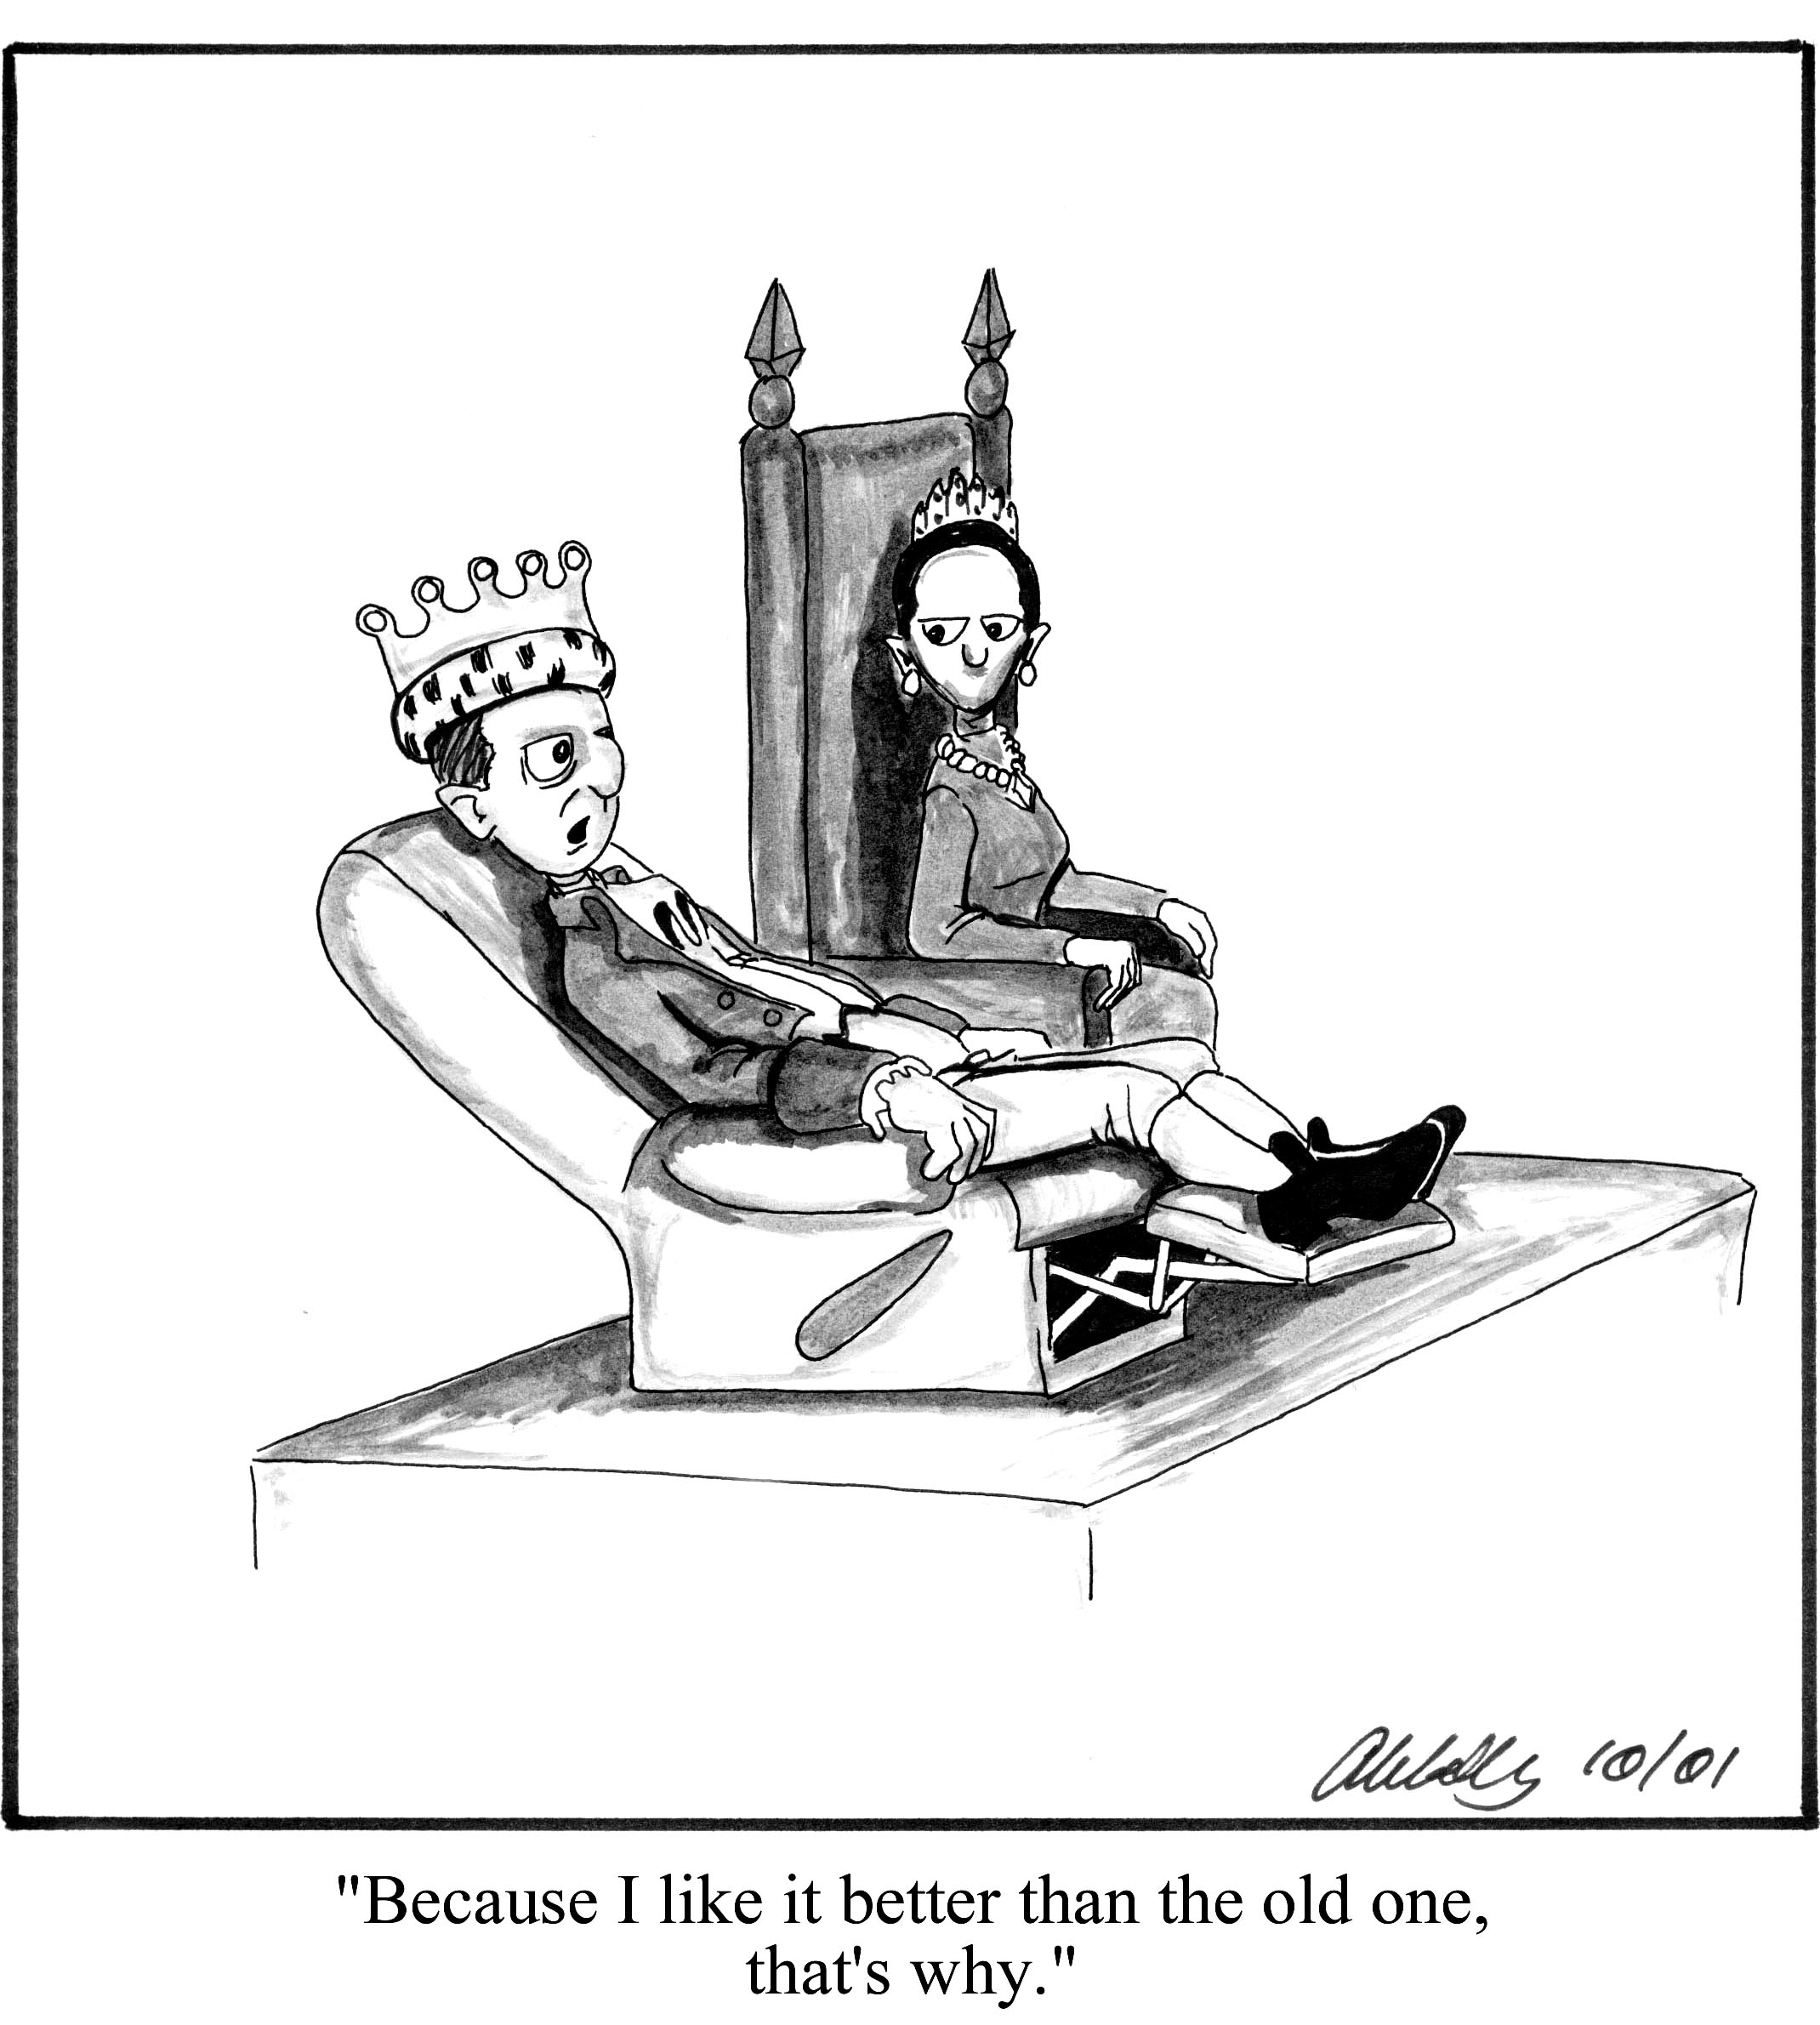
\includegraphics[width=0.5\textwidth]{throneEC.jpg}
  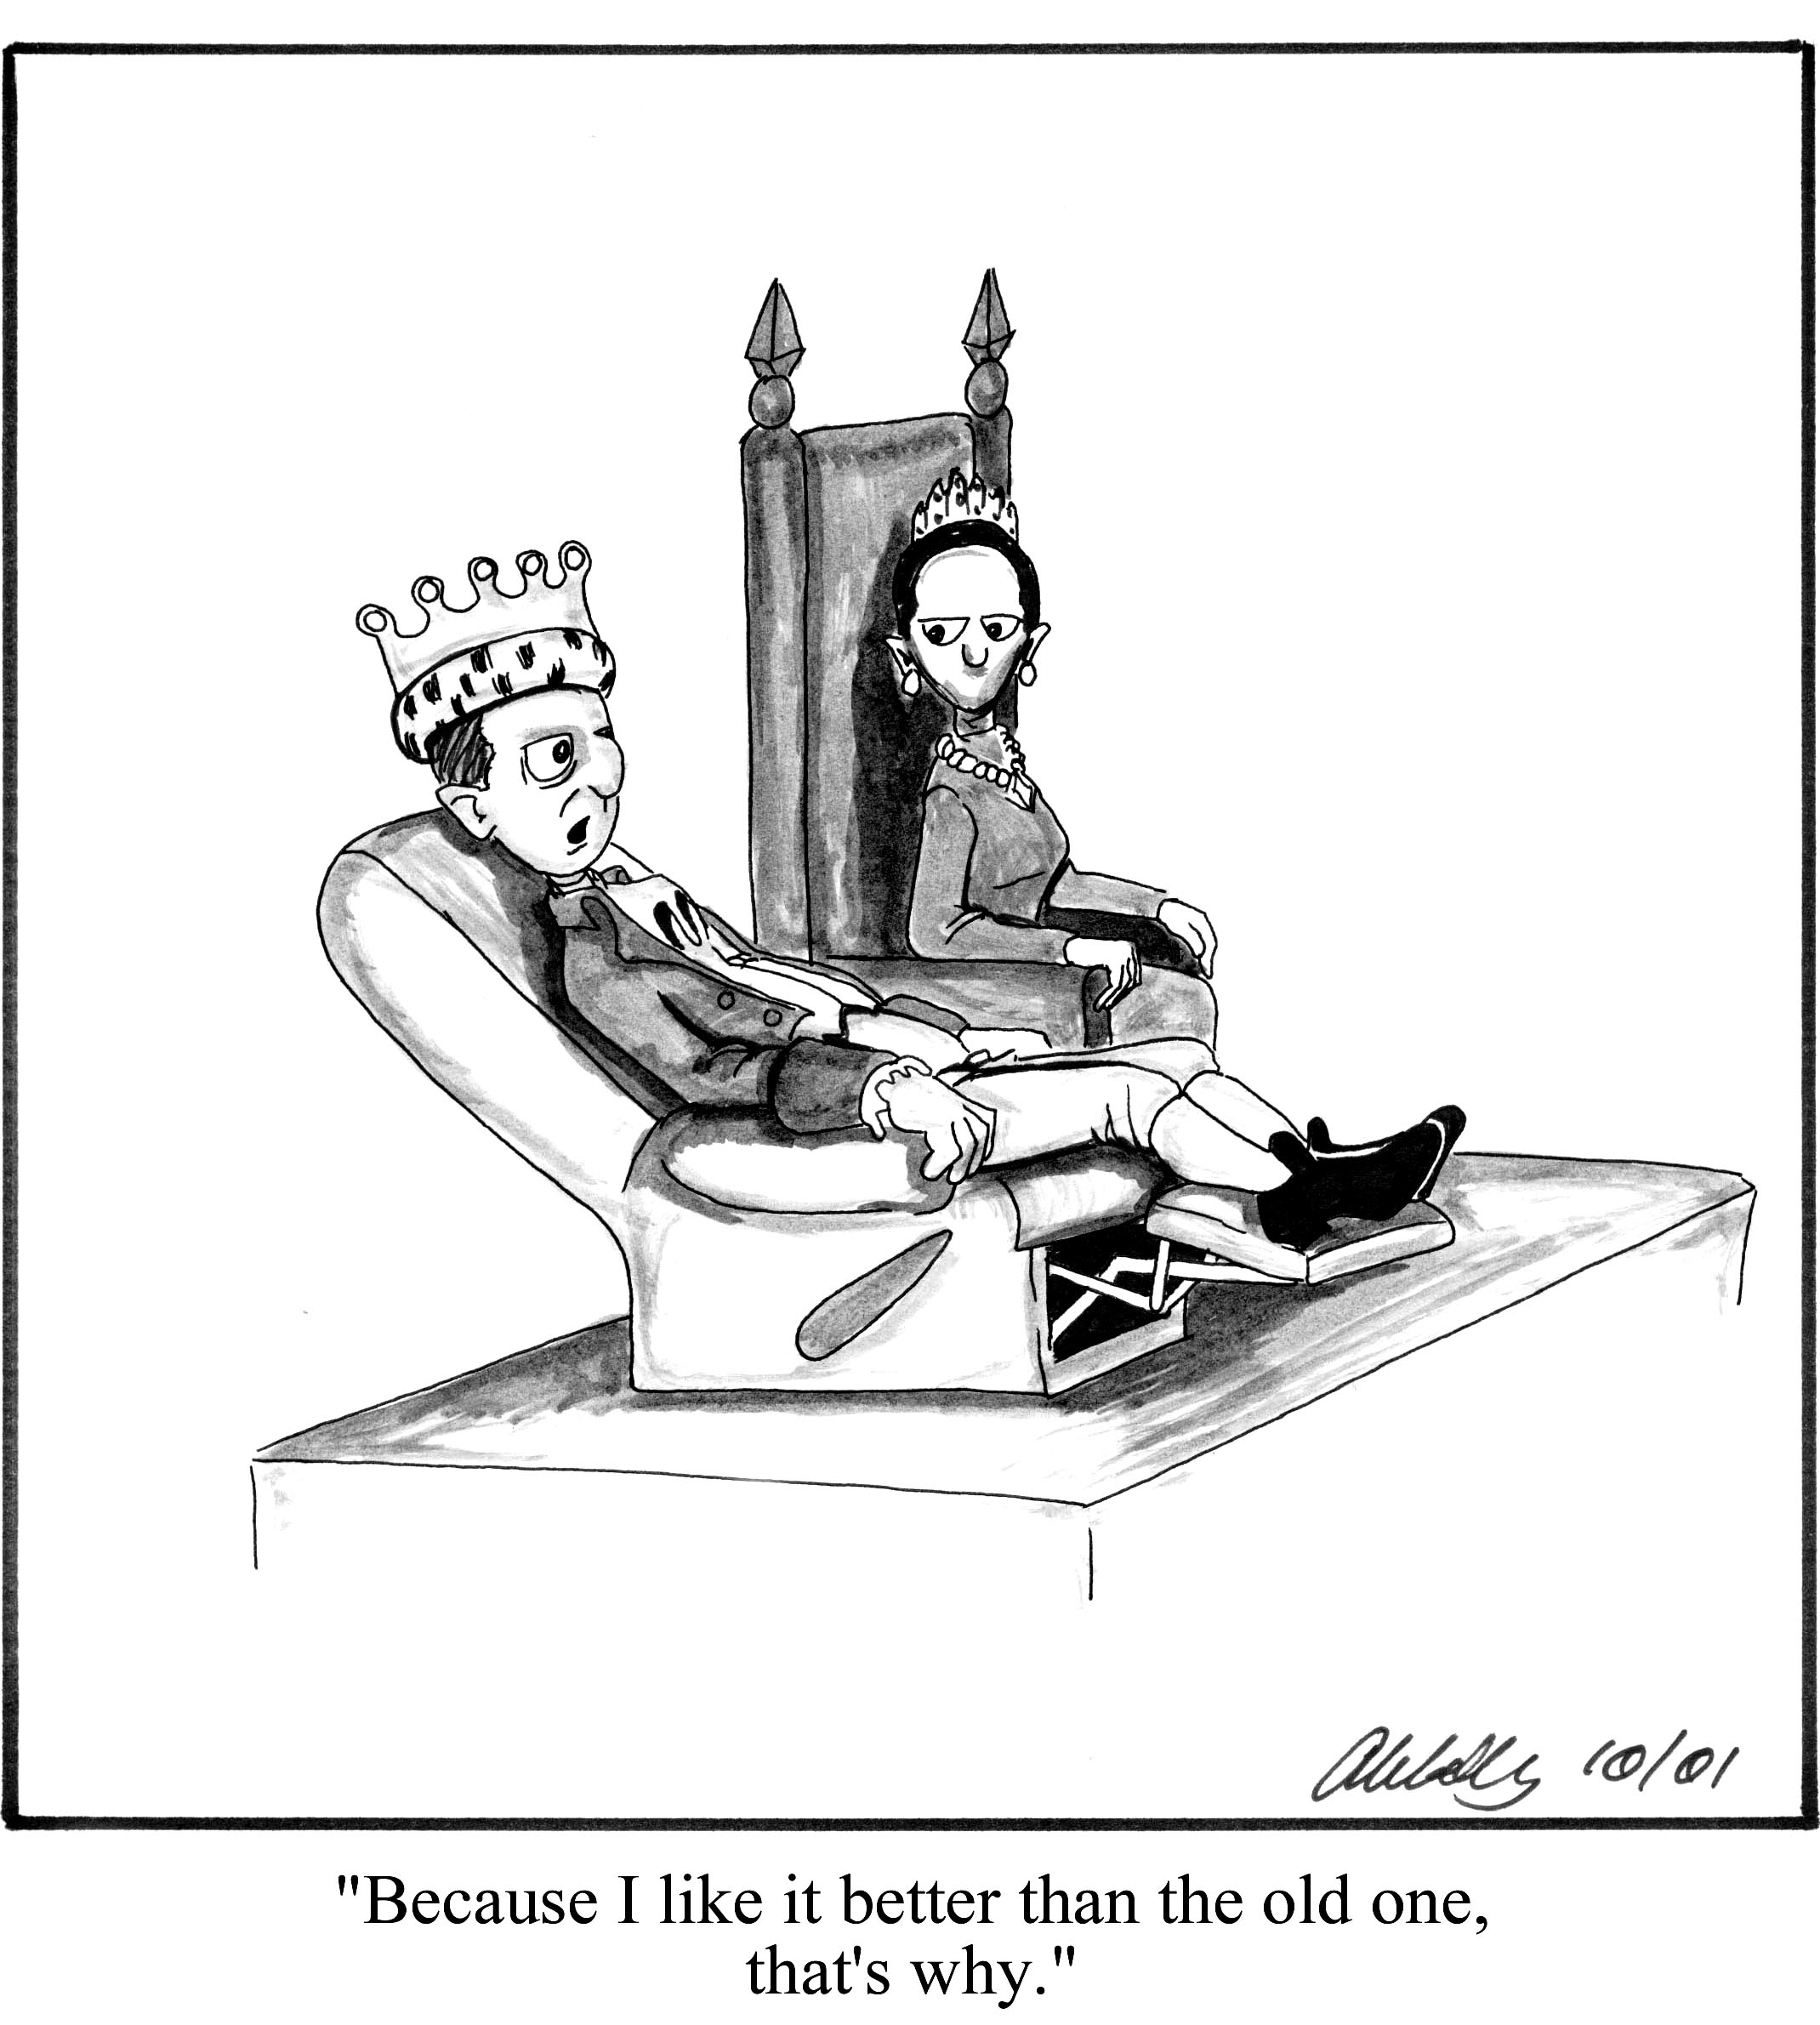
\includegraphics[width=0.3\textwidth]{throneEC.jpg}
  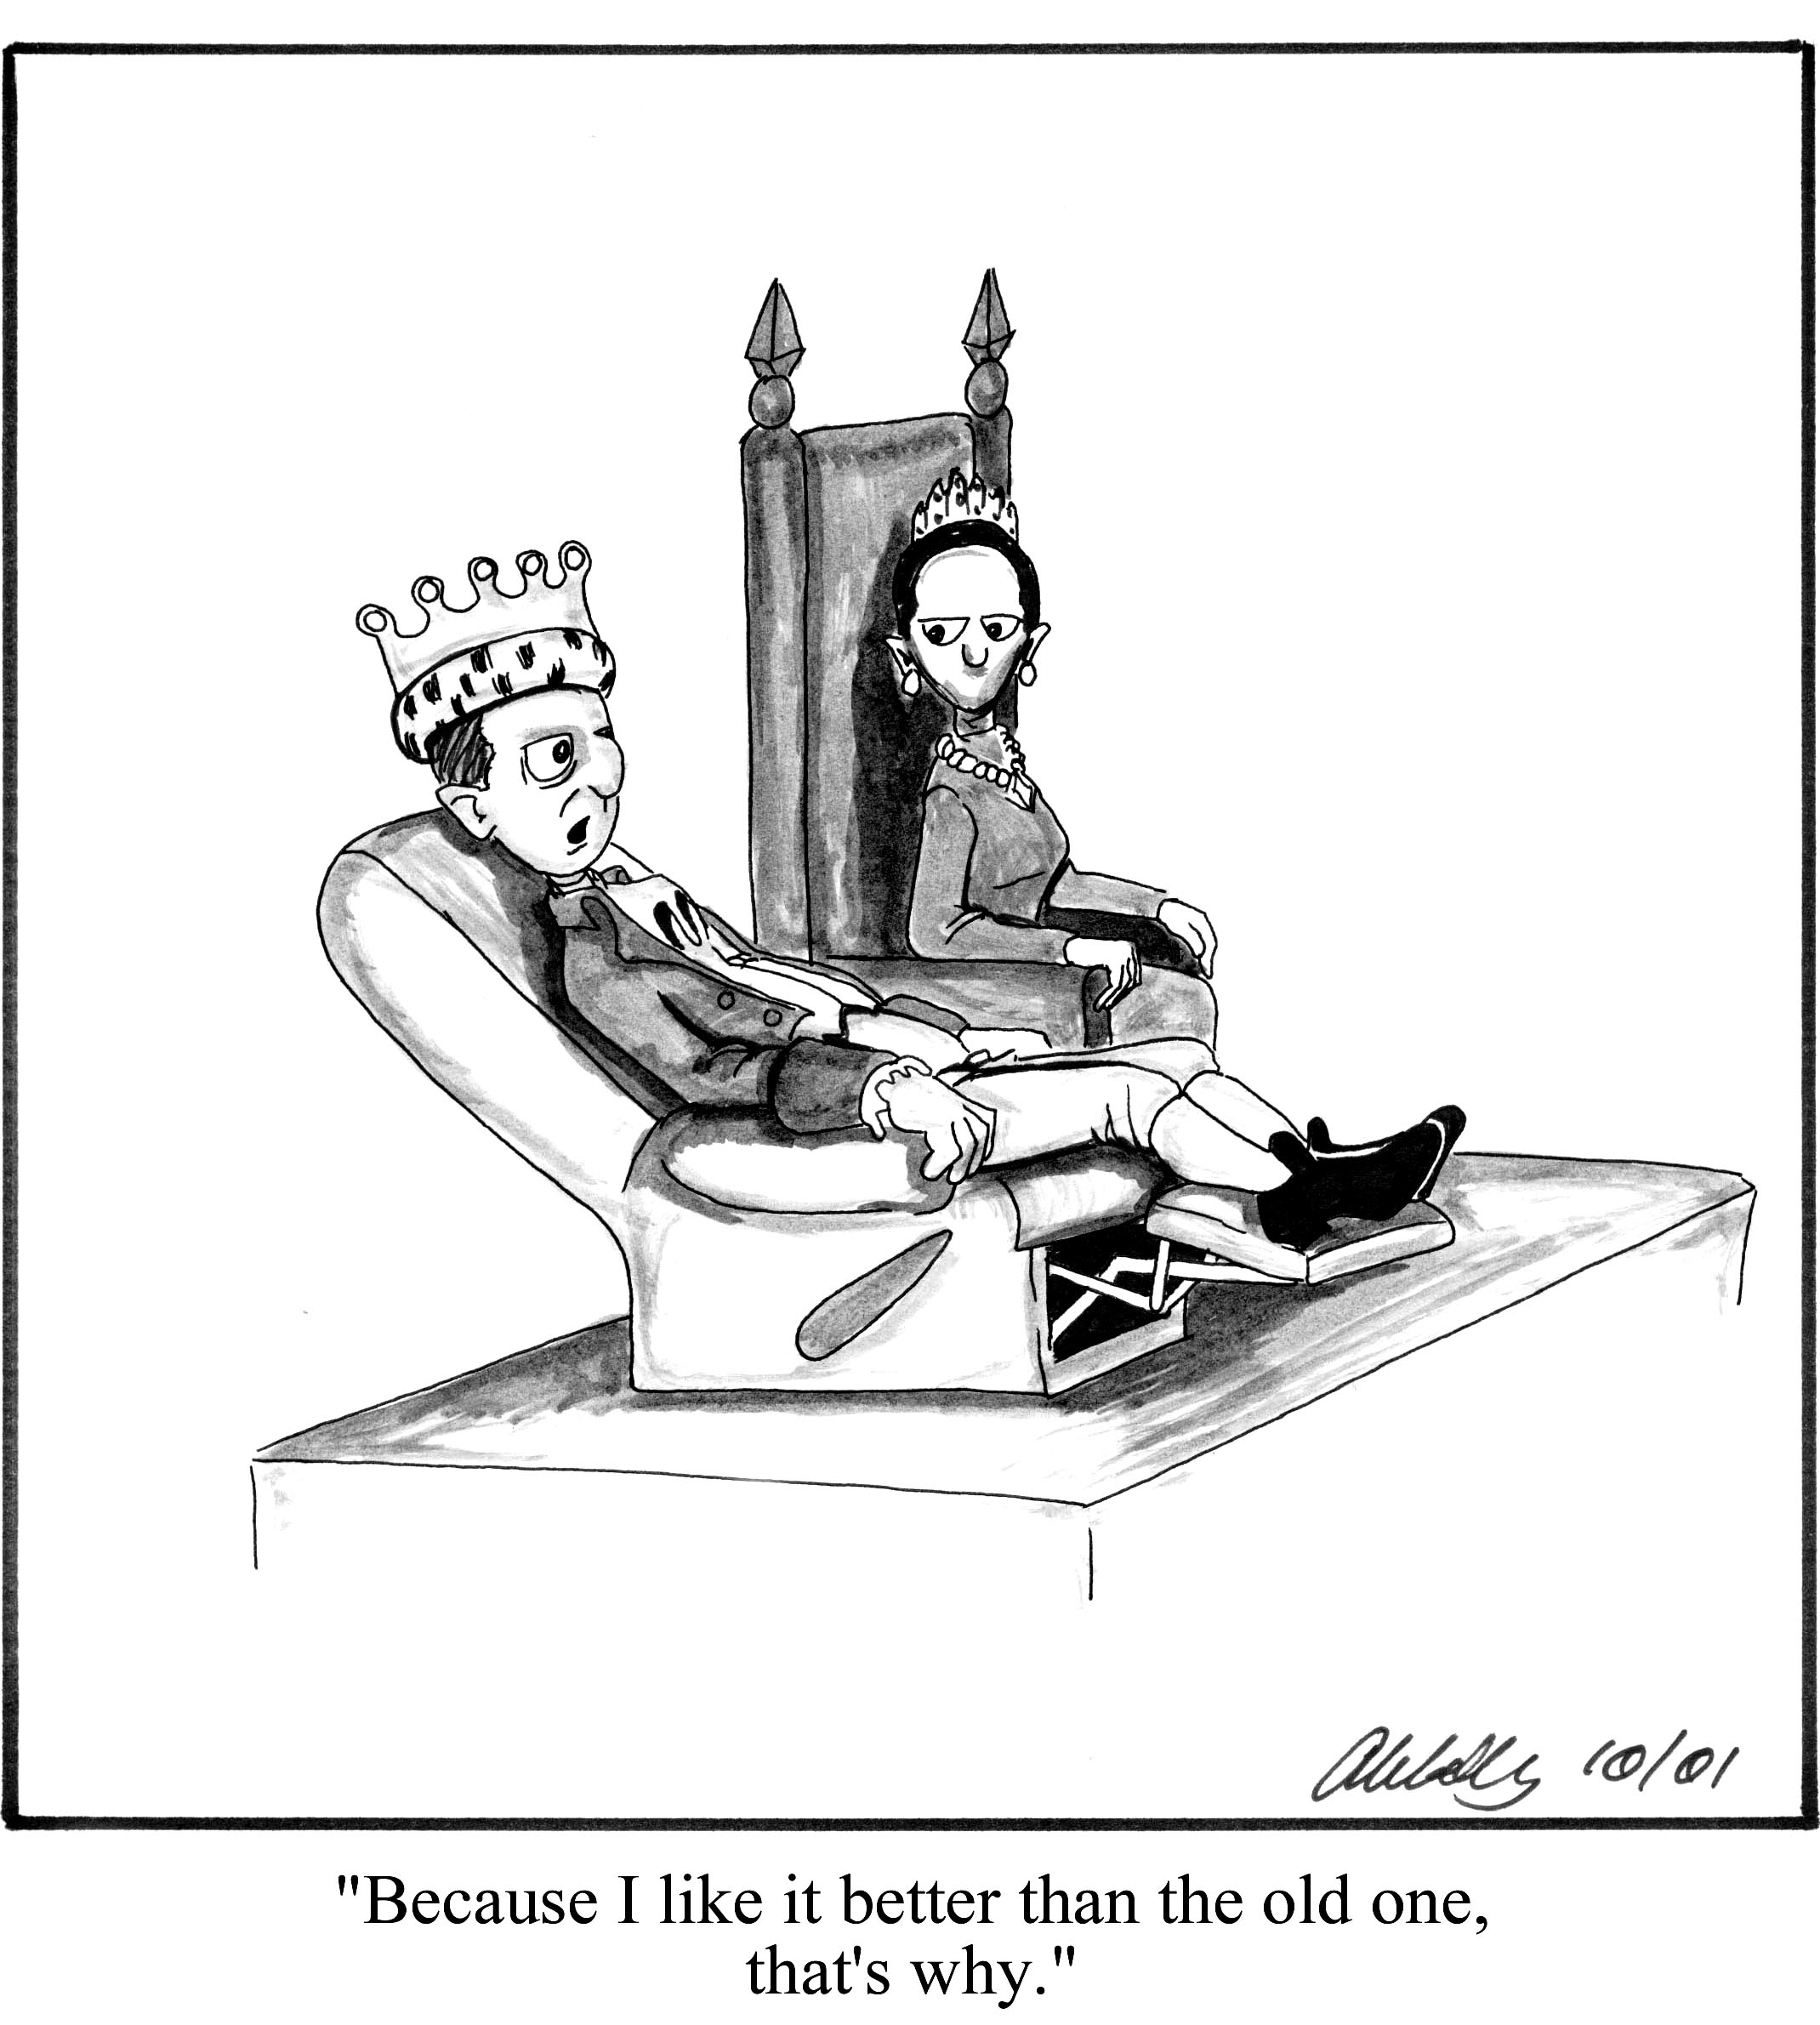
\includegraphics[width=0.15\textwidth]{throneEC.jpg}
\end{verbatim}

\subsection{A Universal Recipe}

\LaTeX\ has a very powerful weapon for reducing the size of almost
anythings. More precisely, it can reduce anything producing what
\LaTeX\ considers a box. This weapon is called
\verb|\scalebox|. Consider an example (check the source of this file
to see how it was produced).

\begin{center}
\begin{tabular}{|c|c|}
\hline \Huge
\begin{tabular}[b]{cr}
year & users \\ \hline
2007 &    47,753 \\
 2008 &    114,494 \\
 2009 &    207,506 \\
 2010 &   371,054 \\
\end{tabular}
&

\includegraphics[width=0.28\textwidth]{chairEC}\\
\hline
\multicolumn{2}{|c|}{The number of users of EasyChair and one of its
  logos,}\\
\multicolumn{2}{|c|}{scaled to the number of users in 2010} \\
\hline
\end{tabular}
\end{center}
This is what happens when we put (almost) the same \LaTeX\ code in 
\verb|\scalebox{0.55923}{...}| to scale it down to the number of users
in 2009:

\begin{center}
\scalebox{0.55923}{%
\begin{tabular}{|c|c|}
\hline \Huge
\begin{tabular}[b]{cr}
year & users \\ \hline
2007 &    47,753 \\
 2008 &    114,494 \\
 2009 &    207,506 \\
 2010 &   371,054 \\
\end{tabular}
&

\includegraphics[width=0.28\textwidth]{chairEC}\\
\hline
\multicolumn{2}{|c|}{The number of users of EasyChair and one of its
  logos,}\\
\multicolumn{2}{|c|}{scaled to the number of users in 2009} \\
\hline
\end{tabular}}
\end{center}
We can scale it down even further to the 2008 figure using
\verb|\scalebox{0.30856}{...}|:

\begin{center}
\scalebox{0.30856}{%
\begin{tabular}{|c|c|}
\hline \Huge
\begin{tabular}[b]{cr}
year & users \\ \hline
2007 &    47,753 \\
 2008 &    114,494 \\
 2009 &    207,506 \\
 2010 &   371,054 \\
\end{tabular}
&

\includegraphics[width=0.28\textwidth]{chairEC}\\
\hline
\multicolumn{2}{|c|}{The number of users of EasyChair and one of its
  logos,}\\
\multicolumn{2}{|c|}{scaled to the number of users in 2008} \\
\hline
\end{tabular}}
\end{center}
or further down to 2007:

\begin{center}
\scalebox{0.12870}{%
\begin{tabular}{|c|c|}
\hline \Huge
\begin{tabular}[b]{cr}
year & users \\ \hline
2007 &    47,753 \\
 2008 &    114,494 \\
 2009 &    207,506 \\
 2010 &   371,054 \\
\end{tabular}
&

\includegraphics[width=0.28\textwidth]{chairEC}\\
\hline
\multicolumn{2}{|c|}{The number of users of EasyChair and one of its
  logos,}\\
\multicolumn{2}{|c|}{scaled to the number of users in 2008} \\
\hline
\end{tabular}}
\end{center}

This size reduction technique is very efficient: using the right scale
you may post your whole article on Twitter in a single tweet. However,
it may also may parts of your text virtually unreadable with an
unfortunate side effect of annoying reviewers. 



\label{sect:bib}
\bibliographystyle{plain}
%\bibliographystyle{alpha}
%\bibliographystyle{unsrt}
%\bibliographystyle{abbrv}
\bibliography{easychair}

%------------------------------------------------------------------------------
\appendix
\section{{\easychair} Requirements Specification}
\label{sect:easychair-requirements}

The following high-level requirements were set for the development of 
the {\easychair} class, and were refined as development went along.

\begin{enumerate}
\item
The style should be easy to use. 
The average {\LaTeX} user should not need to read a long manual.

\item
It should be economical in space but the text should be nice-to-read.

\item
It should use fonts producing a reasonable-quality PDF.

\item
The bibliography should produce hyperlinks.

\item
Sections should produce menu sections in PDF.

\item
The text should look good on both A4 and letter paper.

\item
The style should be single-column for convenience of scrolling.

\item
The print area should be convenient for printing using print-on-demand publishers.

\item
Running heads.
\end{enumerate}

%------------------------------------------------------------------------------
% Index
%\printindex

%------------------------------------------------------------------------------
\end{document}

% EOF
